\chapter{Routing Fundamentals: Part
1}\label{routing-fundamentals-part-1}

\subsection{WHAT IS ROUTING ?}\label{what-is-routing}

ROUTING is the process that routers use to determine the path that IP
packets should take over a network to reach their destination.

\begin{itemize}
\tightlist
\item
  ROUTERS store routes to all their known destinations in a ROUTING
  TABLE
\item
  When ROUTERS receive PACKETS, they look in the ROUTING TABLE to find
  the best route to forward that packet.
\end{itemize}

There are two main routing methods (methods that routers use to learn
routes):

\begin{itemize}
\tightlist
\item
  DYNAMIC ROUTING : ROUTERS use Dynamic Routing Protocols (ie: OSPF) to
  share routing information with each other automatically and build
  their routing tables.
\item
  STATIC ROUTING : A network engineer / Admin manually configures routes
  on the router.
\end{itemize}

A ROUTE tells the ROUTER :

\begin{itemize}
\tightlist
\item
  to send a packet to Destination X, you should send the pack to
  \textbf{\emph{next-hop}} Y
\item
  or if the Destination is directly connected to the router, \emph{send
  the packet directly to the destination.}
\item
  or if the Destination is the router's own IP address, \emph{receive
  the packet for yourself (don't forward it).}
\end{itemize}

\begin{figure}
\centering
\pandocbounded{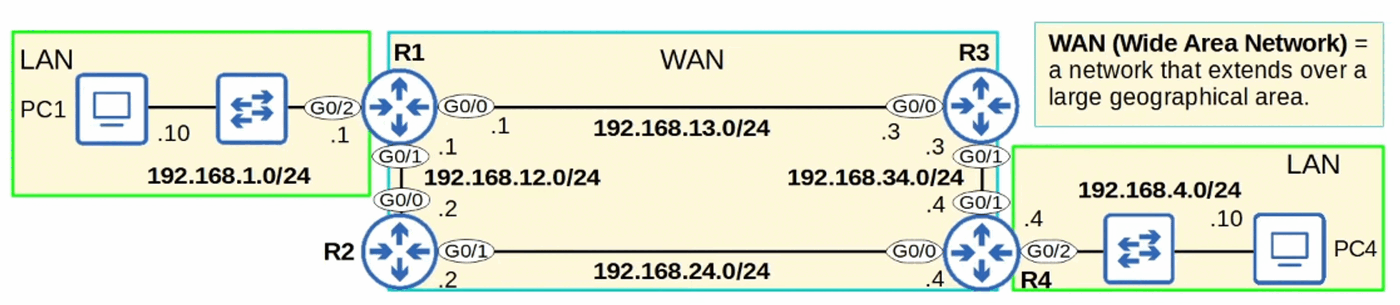
\includegraphics[keepaspectratio,alt={image}]{images/11-routing-fundamentals-part1/img-001.png}}
\end{figure}

WAN (Wide Area Network) = network that extends over a large geographic
area.

\begin{figure}
\centering
\pandocbounded{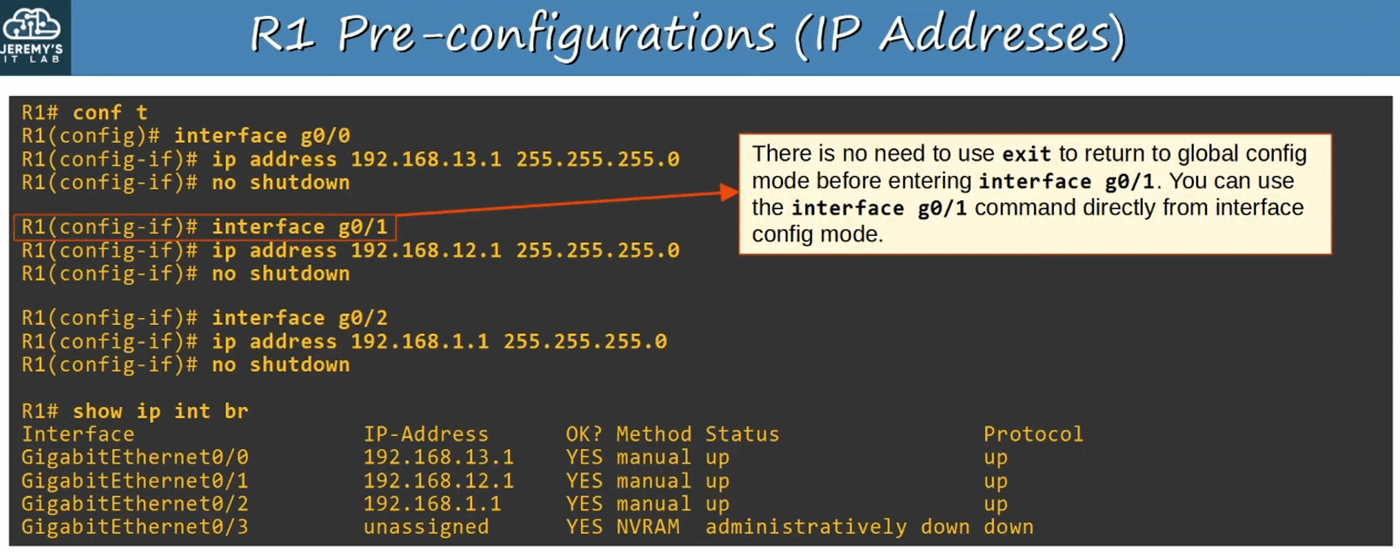
\includegraphics[keepaspectratio,alt={image}]{images/11-routing-fundamentals-part1/img-002.png}}
\end{figure}

\begin{figure}
\centering
\pandocbounded{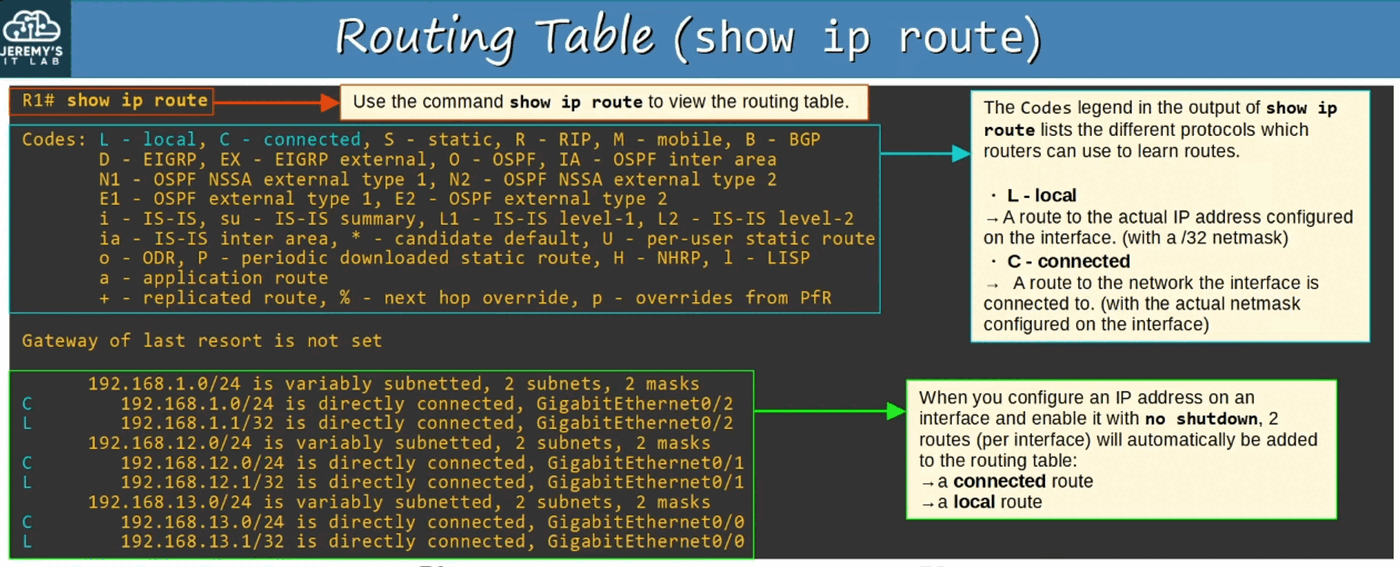
\includegraphics[keepaspectratio,alt={image}]{images/11-routing-fundamentals-part1/img-003.png}}
\end{figure}

\begin{figure}
\centering
\pandocbounded{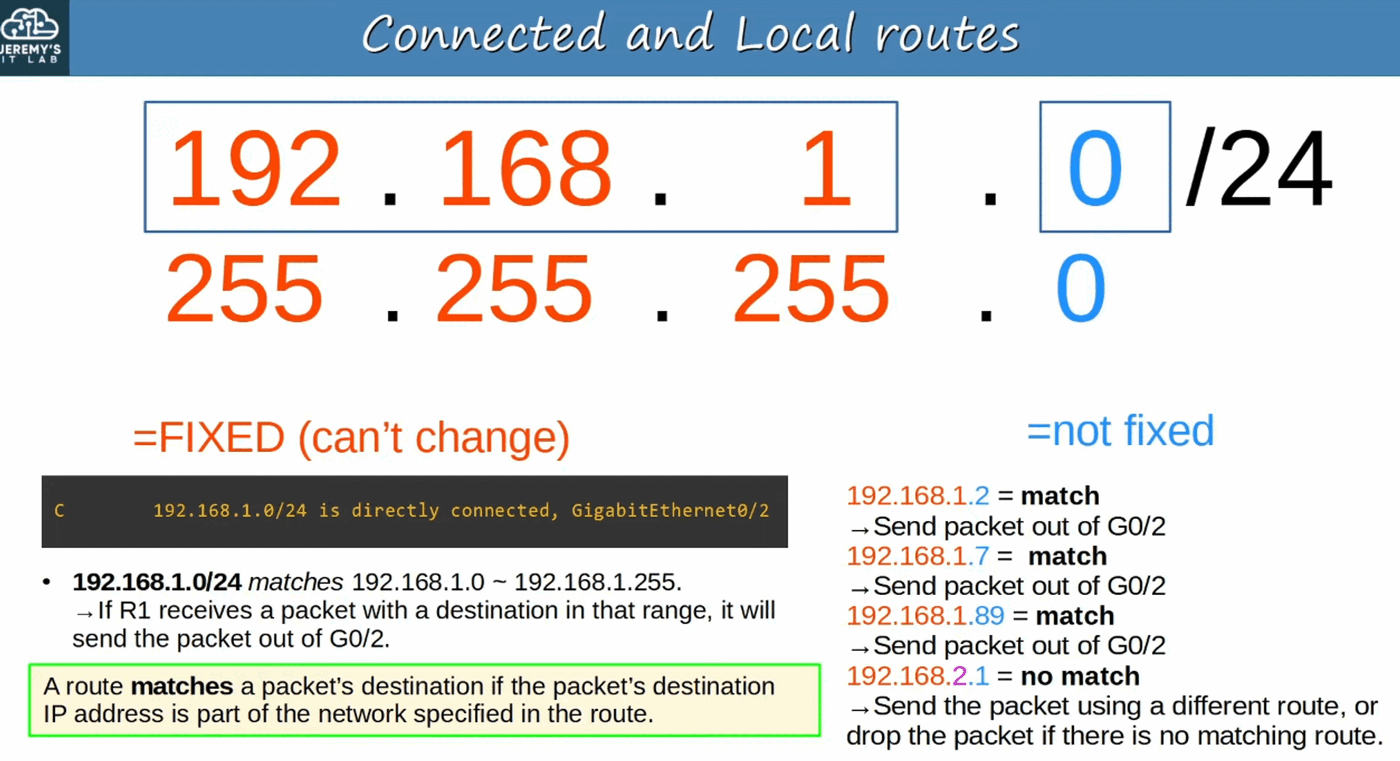
\includegraphics[keepaspectratio,alt={image}]{images/11-routing-fundamentals-part1/img-004.png}}
\end{figure}

\begin{figure}
\centering
\pandocbounded{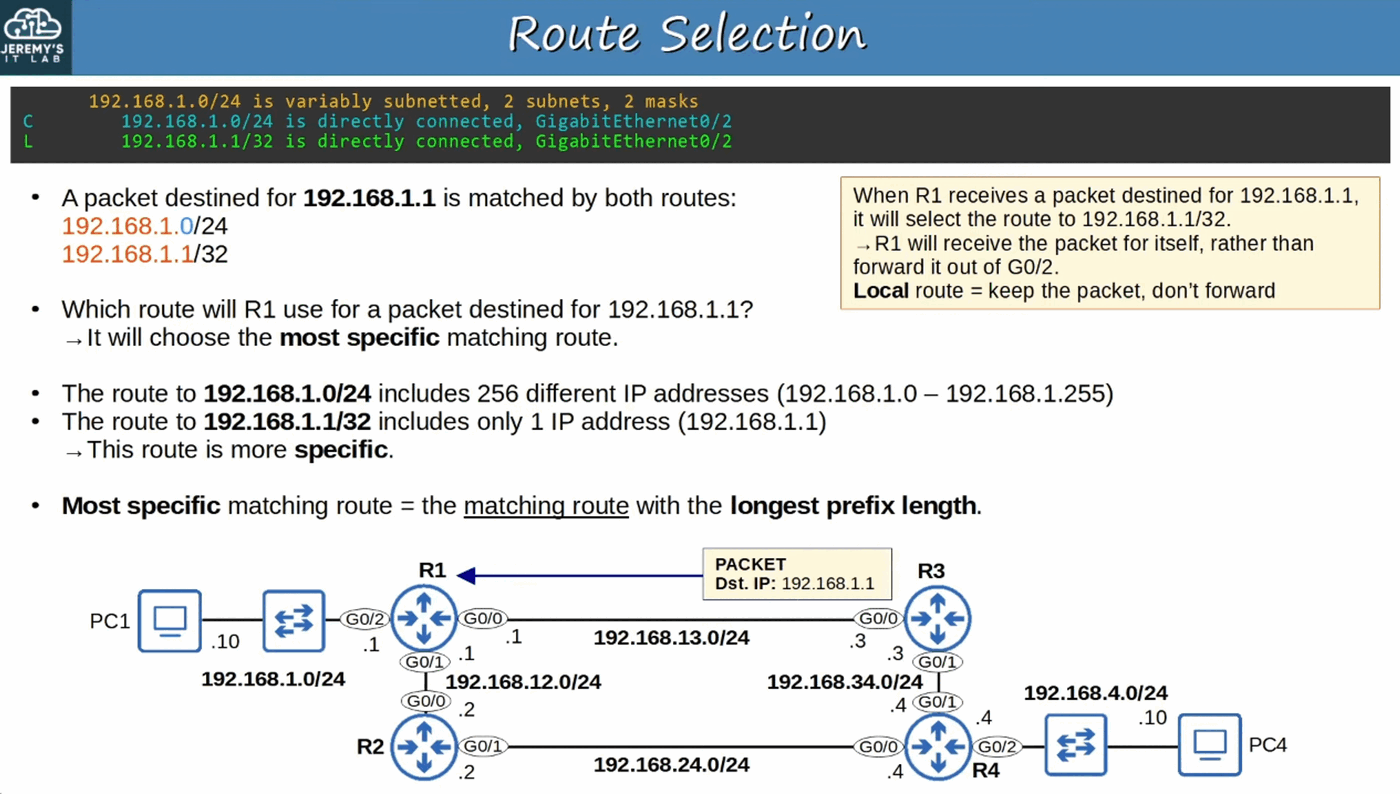
\includegraphics[keepaspectratio,alt={image}]{images/11-routing-fundamentals-part1/img-005.png}}
\end{figure}

\begin{figure}
\centering
\pandocbounded{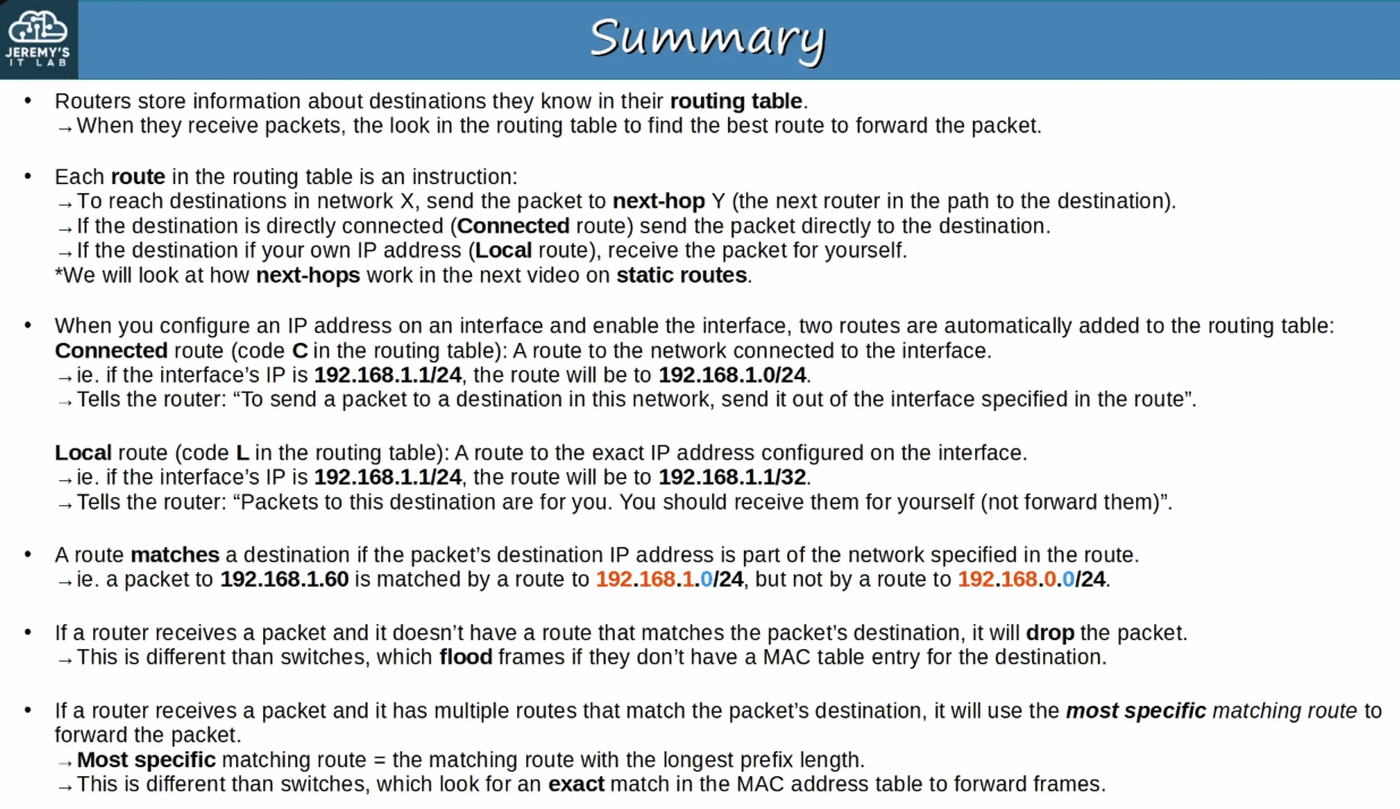
\includegraphics[keepaspectratio,alt={image}]{images/11-routing-fundamentals-part1/img-006.png}}
\end{figure}
